\subsection{Brown Cluster}
    Der fertige Prototyp verwendet zum erstellen der benötigten Wortklassen eine Implementierung des \emph{Brown clustering} Algorithmus von Percy Liang. Dennoch habe ich mich im Laufe dieser Arbeit lange mit der Implementierung eines \emph{Brown clustering} Algorithmus auseinandergesetzt.
    
    Im Folgenden werden die unternommen Versuche in ihrer zeitlichen Abfolge dargestellt. Die Ansätze werden nur Oberflächlich erklärt. Damit soll gezeigt werden welche Probleme zur Verwendung einer \emph{third party} Lösung geführt haben.
        
    \subsubsection*{1. Versuch}

  		\cite{speechcommunication:exchange} versprechen im Abstract ihres Berichts eine \enquote{effiziente Methode zur Erzeugung von Wort Klassen} (S. 19). Hierzu beschreiben sie in Abschnitt 2.3 einen \emph{exchange algorithm}. Dabei wird zu Beginn den \emph{G} häufigsten Worten eine eigene Klasse zugeteilt. Bei \emph{G} handelt es sich um die gewünschte Anzahl an Wortklassen. Die restlichen Worte werden in einer weiteren Klasse zusammengefasst. Nun wird jedes Wort testweise von seiner bisherigen in jede andere Klasse verschoben. Für diese Verteilung wird dann jeweils die \emph{log-likelihood} (siehe \autoref{sec:brownClustering}) berechnet. Am Ende landet das Wort in der Klasse, die zu der niedrigsten \emph{log-likelihood} führt. Dieser Prozess wird so lange wiederholt bis keine optimierung durch verschieben mehr erreicht werden kann oder eine bestimmte Anzahl an Iterationen überschritten wurde.
            
		\begin{figure}[H]
			\centering
  			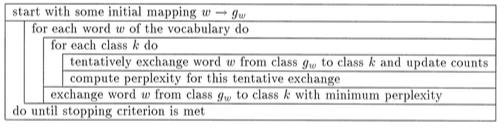
\includegraphics[width=.8\linewidth]{images/exchangeAlg.png}
  			\caption{\emph{} \parencite[S. 24 Abb. 1 ]{speechcommunication:exchange}}				
			\label{fig:exchangeAlgorythm}
		\end{figure}

		Damit die Werte zur Berechnung der \emph{log-likelihood} nicht nach jedem Verschieben eines Wortes aufwändig neu aus dem \emph{Corpus} genereiert werden müssen, werden die betreffenden Werte durch Addition bzw. Substraktion aktualisiert. \parencite[S. 26 f. Abschnitt 3.1.2]{speechcommunication:exchange}
            
        \newpage
        \begin{lstlisting}[caption=Beispiel für das Aktualisieren von \emph{counts} nachdem ein Wort zu einer Klasse hinzugefügt wurde.,label=code:countUpdate, captionpos=b]
for group in predecessor_groups_of[word]:
	if group != new_group:
        group_bigramm_counts[(group, new_group)] += succsessor_word_count_of_group[group][word]
 
for group in self.succsessor_groups_of[word]:
	if group != new_group:
        group_bigramm_counts[(new_group, group)] += predecessor_word_count_of_group[group][word]
        \end{lstlisting}
  
		In den ersten Versionen der Implementierung entstanden hier oft fehler. Um diese Fehler leichter zu finden wurden Tests für die update Funktionen geschrieben. Dazu wurde ein sehr kleiner \emph{Corpus} verwendet bei dem die Effekte einer Verschiebung leicht manuell zu berechnen waren. In \autoref{code:testCounts} kommt \texttt{Altweibersommer} zwei mal im \emph{Corpus} vor also sollte der \texttt{group\_count} von Gruppe \texttt{0} um zwei erhöhen. Die \texttt{group\_bigramm\_counts} lassen sich ebenso aus de

		\begin{lstlisting}[caption=Beispiel eines Tests zum Aktualisieren von \emph{counts} nachdem ein Wort einer Klasse hinzugefügt wurde., captionpos=b, label=code:testCounts]
                
def test_move_Altweibersommer_to_gruop_0(learner, group_bigramm_counts, group_counts):
    (temp_group_bigramm_counts, temp_group_counts) = learner.move_word_to_group("Altweibersommer", 0)

    group_counts[0]              += 2
    group_bigramm_counts["0_1"]  += 1
    group_bigramm_counts["0_17"] += 1
    group_bigramm_counts["0_0"]  += 2

    for group in group_counts:
        assert group_counts[group] is temp_group_counts[group]
    for bigram in group_bigramm_counts:
        assert group_bigramm_counts[bigram] is temp_group_bigramm_counts[bigram]
		\end{lstlisting}
                
		So kann sichergestellt werden, dass die \emph{counts} auch bei eventuellen zukünftigen Optimierungen richtig aktualisiert werden. Dabei werden nicht nur die Werte für die veränderten \emph{counts} (\texttt{0\_1}, \texttt{0\_17}, \texttt{0\_0} und \texttt{group\_counts[0]}) überprüft, sondern die gesammte Tabelle. Damit tritt auch das Aktualisieren von falschen Werten als Fehler im Test auf. Rückblickend müssten hier die \emph{counts} allerdings neu gezählt und dann mit den Aktualisierungen verglichen werden. In der letzten Version von \autoref{code:countUpdate} befanden sich immer noch Fehler.
		\newpage

		Diese Tests können natürlich auch nicht gegen Fehlinterpretationen des Algorithmus absichern. Die einzige Verifizierung einer korrektem Implementierung sind sinnvoll generierte Wortklassen. Für diese wird ein ausreichend großer \emph{Corpus} benötigt. Allerdings konnte mit der umgesetzten Implementierung keine zufriedenstellende Laufzeit für einen entsprechend großen \emph{Corpus} erreicht werden.

	\subsubsection*{2. Versuch}
        							
		\cite{cumpatationalLinguistics:classBasedNGramms} gehen zwar im Vergleich zu \cite{speechcommunication:exchange} weitaus weniger auf eine konkrete Implementierung ein, dafür finden sich hierzu offen zugängliche Implementierungen auf \emph{github.com}. Beispielsweise von \emph{percyliang} (\url{https://github.com/percyliang/brown-cluster}, besucht am 20.06.2015), von \emph{mheilman} (\url{https://github.com/mheilman/tan-clustering}, besucht am 20.06.2015) und von \emph{HaohanWang} (\url{https://github.com/HaohanWang/BrownClustering}, besucht am 20.06.2015).
            
		Alle drei basieren laut Eigenaussage auf \cite{cumpatationalLinguistics:classBasedNGramms} Allerdings wurden bei \emph{mheilman}'s Version einige Abwandlungen am Algorithmus vorgenommen. \emph{HaohanWang}'s Lösung ist hierbei die kürzeste und am wenigsten Umfangreiche. Dies schien am besten geeignet um den Algorithmus zu verstehen und später möglicherweise weiter zu optimieren. 
            
		Nach beheben verschiedener Fehler im Code von \emph{HaohanWang} war es möglich mit einem kleinen Test \emph{Corpus} intuitiv sinnvolle Ergebnisse zu erzielen.
        \newline
            
        \begin{figure}[H]
			\centering
            \begin{subfigure}{.45\textwidth}
                \centering
  				\texttt{
                the cat chased the mouse \linebreak
  				the dog chased the cat \linebreak
  				the mouse chased the dog}
                \caption{Corpus}
            \end{subfigure}
            \begin{subfigure}{.45\textwidth}
                \centering
                \begin{tabular}{ c | c | c }
                	Klasse 1 & Klasse 2 & Klasse 3 \\ \hline
                    the & chased & cat, dog, mouse \\
                \end{tabular}
  				\caption{Klassen}
            \end{subfigure}
            \caption{Klassifizierung mit überarbeitetem code von \emph{HaohanWang}}
			\label{fig:clusterCatDogAndMouse}
		\end{figure}

		Diese Einordnung lässt sich Erklären, da \texttt{cat}, \texttt{mouse}, und \texttt{dog} immer den gleichen Vorgänger und fast immer den gleichen Nachfolger haben.


		Auch wenn \emph{HaohanWang} das in \autoref{sec:brownClustering} beschriebene \enquote{Fenster} implementiert, so wird hier die \emph{Qualität} immer noch für jede mögliche Vereinigung von 2 Klassen teuer neu berechnet. Dies führt auch schon bei einem sehr kleinen \emph{Corpus} von wenigen 100 Wörtern zu sehr langen Laufzeiten.
	
    \newpage
	\subsubsection*{3. Versuch}
    \label{sec:thirdTry}
        \emph{percyliang} verweist in der \emph{README} seiner Implemetierung auf seine Masterarbeit \parencite{percyliang:meng}. In dieser beschreibt er ab S. 43 auch die Implementierung des \emph{Brown clustering} Algorithmus. Er benutzt dazu die Metapher eines Graphs. In erster Linine beschreibt er eine Tabelle \emph{L(cc')}. In dieser wird, für alle möglichen Kombinationen, der potenzielle Einfluss einer Vereinigung von 2 Klassen auf die endgültige Qualität gespeichert. \parencite[S. 47]{percyliang:meng}
  
		Diese Werte werden laut Liang einmal initial berechnet. Nach der Vereinigung von 2 Klassen können viele dieser Werte dann durch Additionen aktualisiert werden und nur manche müssen neu berechnet werden. 

		Leider geht Liang in seiner Arbeit zwar stark auf die Komplexität aber weniger auf die konkrete Implementierung ein. In einem Versuch der Umsetzung nach Liang gelang es den Graph sowie die Tabelle \emph{L(cc')} initial zu berechnen. Nach Problemen mit der Aktualisierung der Tabelle erschien es sinnvoller auf die fertige Version von Liang zurückzugreifen. Diese ist in \emph{C++} geschrieben und verarbeitet \emph{Corpi} für welche der Code aus Versuch 1 und Versuch 2 über 5h benötigten in Sekunden. 